\documentclass[14pt,a4paper]{extarticle}
\usepackage[T1]{fontenc}
\usepackage[utf8]{inputenc}
\usepackage[scaled]{helvet}
\renewcommand{\familydefault}{\sfdefault}
\usepackage{amsmath}
\usepackage{sansmath}
\sansmath
\usepackage[a4paper,margin=2cm]{geometry}
\usepackage{tikz}
\usetikzlibrary{angles,quotes,patterns}
\usepackage{array}
\pagestyle{empty}
% Zweite Seite: 5-mm-Kästchen, 1 cm Rand
\newcommand{\kaestchen}{\newpage\null\begin{tikzpicture}[remember picture,overlay]
\begin{scope}[shift={(current page.south west)}]\draw[step=5mm, black!45, line width=0.3pt] (1cm,1cm) grid (20cm,28.5cm);\draw[black!45, line width=0.3pt] (1cm,1cm) rectangle (20cm,28.5cm);\end{scope}
\end{tikzpicture}}
\setlength{\parindent}{0pt}
\hyphenpenalty=10000

% Nur Schwarz und Grau, die Blätter werden schwarz-weiß kopiert.
% Merkblock: Begriff und Text links, Zeichnung rechts.
\newcommand{\bl}{0.5}
\newcommand{\block}[3]{%
\begin{minipage}[c]{\bl\textwidth}\raggedright{\Large\bfseries #1\par}\medskip #2\end{minipage}\hfill
\begin{minipage}[c]{\dimexpr0.97\textwidth-\bl\textwidth\relax}\centering #3\end{minipage}\par}

\renewcommand{\bl}{0.55}
\usepackage{enumitem}
\setlist[enumerate]{nosep,leftmargin=1.5em}
\begin{document}

{\LARGE\bfseries Wiederholung\par}
\vspace{0.3cm}

\block{Parallel und senkrecht}{%
Parallele Geraden haben überall den gleichen Abstand und schneiden sich nie: $f \parallel g$\par\medskip
Senkrechte Geraden bilden einen rechten Winkel: $f \perp h$}{%
\begin{tikzpicture}[scale=0.85]
  \draw[thick] (-2.2,0.8) -- (2.2,0.8) node[right] {$f$};
  \draw[thick] (-2.2,-0.8) -- (2.2,-0.8) node[right] {$g$};
  \draw[very thick, gray] (-0.8,-1.6) -- (-0.8,1.7) node[above] {$h$};
  \draw (-0.8,0.8) rectangle (-0.5,1.1);
\end{tikzpicture}}

\vspace{0.3cm}

\block{Teile eines Winkels}{%
Ein Winkel hat einen Scheitelpunkt $S$, zwei Schenkel und einen Winkelbogen. Man benennt ihn mit einem griechischen Buchstaben: $\alpha$ (Alpha), $\beta$ (Beta), $\gamma$ (Gamma), $\delta$ (Delta).}{%
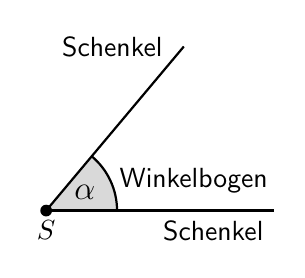
\begin{tikzpicture}[scale=0.85]
  \coordinate (S) at (0,0); \coordinate (A) at (3.4,0); \coordinate (B) at (50:3.2);
  \pic[fill=gray!30, draw=black, thick, angle radius=0.9cm, "\large$\alpha$", angle eccentricity=0.6] {angle=A--S--B};
  \draw[thick] (S) -- (A) node[below left] {Schenkel};
  \draw[thick] (S) -- (B) node[left=4pt] {Schenkel};
  \fill (S) circle (2.5pt) node[below] {$S$};
  \node[right] at (25:1.05) {Winkelbogen};
\end{tikzpicture}}

\vspace{0.3cm}

{\Large\bfseries Winkelarten\par}
\medskip
\newcommand{\wa}[1]{\begin{tikzpicture}[scale=0.42]\fill[gray!35] (0,0) -- (0:0.9) arc (0:#1:0.9) -- cycle;\draw[thick] (1.6,0) -- (0,0) -- (#1:1.6);\fill (0,0) circle (2pt);\end{tikzpicture}}
\begin{tabular}{@{}*{4}{>{\centering\arraybackslash}p{3.85cm}}@{}}
\wa{50} & 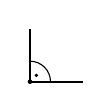
\begin{tikzpicture}[scale=0.42]\draw (0.62,0) arc (0:90:0.62); \fill (45:0.27) circle (1.6pt);\draw[thick] (1.6,0) -- (0,0) -- (0,1.6);\fill (0,0) circle (2pt);\end{tikzpicture} & \wa{130} & \wa{250}\\
spitz & rechter Winkel & stumpf & überstumpf\\
$0^\circ<\alpha<90^\circ$ & $\alpha = 90^\circ$ & $90^\circ<\alpha<180^\circ$ & $180^\circ<\alpha<360^\circ$
\end{tabular}

\vspace{0.3cm}

\block{Winkel messen}{%
\begin{enumerate}
\item Nullpunkt des Geodreiecks auf den Scheitelpunkt.
\item 0-Linie auf einen Schenkel. Zu kurze Schenkel vorher verlängern.
\item Auf der Skala ablesen, die an diesem Schenkel bei $0^\circ$ beginnt. Mit der Winkelart prüfen.
\end{enumerate}}{%
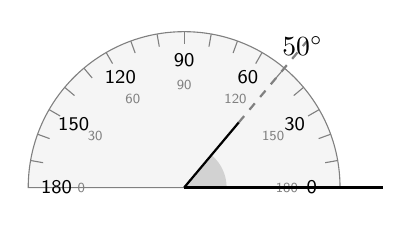
\begin{tikzpicture}[scale=0.9]
  \fill[gray!8] (2.2,0) arc (0:180:2.2) -- cycle; \draw[gray] (2.2,0) arc (0:180:2.2) -- cycle;
  \foreach \a in {0,10,...,180} \draw[gray] (\a:2.2) -- (\a:2.02);
  \foreach \a in {0,30,...,180} \node[font=\scriptsize] at (\a:1.8) {\a};
  \foreach \a/\b in {0/180,30/150,60/120,90/90,120/60,150/30,180/0} \node[gray, font=\tiny] at (\a:1.45) {\b};
  \fill[gray!35] (0,0) -- (0:0.6) arc (0:50:0.6) -- cycle;
  \draw[thick] (0,0) -- (2.8,0); \draw[thick] (0,0) -- (50:1.2); \draw[thick, dashed, gray] (50:1.2) -- (50:2.7);
  \node[font=\bfseries] at (50:2.6) {$50^\circ$};
\end{tikzpicture}}

\vspace{0.3cm}

\block{Winkel zeichnen}{%
\begin{enumerate}
\item Einen Schenkel zeichnen, Scheitelpunkt $S$ markieren.
\item Geodreieck anlegen: Nullpunkt auf $S$, 0-Linie auf den Schenkel.
\item Bei der Gradzahl einen Punkt markieren. Richtige Skala!
\item $S$ mit dem Punkt verbinden, Winkelbogen zeichnen, beschriften.
\end{enumerate}}{%
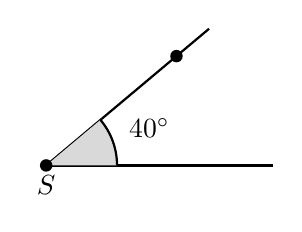
\begin{tikzpicture}[scale=0.9]
  \coordinate (S) at (0,0); \coordinate (A) at (3.2,0); \coordinate (B) at (40:3);
  \draw[thick] (S) -- (A); \draw[thick] (S) -- (B);
  \pic[fill=gray!30, draw=black, thick, angle radius=0.9cm, "$40^\circ$", angle eccentricity=1.55] {angle=A--S--B};
  \fill (0,0) circle (2.5pt) node[below] {$S$};
  \fill (40:2.4) circle (2.5pt);
\end{tikzpicture}}

\vspace{0.3cm}

{\Large\bfseries Aufgaben im Heft\par}
\medskip
Buch S.\,225 Nr.\,74 \qquad S.\,232 Nr.\,92, 93, 94 \qquad S.\,233 Nr.\,95, 96
\kaestchen
\end{document}
